% !TeX program = LuaLaTeX
% !TeX encoding = UTF-8
\documentclass[aspectratio=169, 15pt,usenames,dvipsnames]{beamer}
% Source sans

\usepackage[utf8]{inputenc}
\usepackage{fontspec}
% \usepackage{sansmathfonts}
\usepackage{xcolor}
\usepackage{fontenc}
\usepackage{unicode-math}
\usepackage{listings}
\usepackage{cprotect}
\usepackage{pgfpages}

\usepackage[makeroom]{cancel}

\usefonttheme{serif}
\usefonttheme{professionalfonts}


\usepackage[scaled=1.1]{sourcecodepro}
\usepackage{sourcecodepro}
\usepackage{graphicx}
\usetheme{Madrid}
\usecolortheme{beaver}
% \usepackage{themes/gd/beamerthemegd}
% \usepackage{themes/gd/beamerinnerthemegd}
% \usepackage{themes/gd/beamerouterthemegd}
% \usepackage{themes/gd/beamercolorthemegd}
\let\OLDitemize\itemize
\renewcommand\itemize{\OLDitemize\addtolength{\itemsep}{7pt}}
\setbeamertemplate{itemize items}[circle]
\setbeamertemplate{navigation symbols}{}%remove navigation symbols
\setbeamercolor{itemize item}{fg=black}
\setbeamercolor{itemize subitem}{fg=black}
\setbeamercolor{itemize subsubitem}{fg=black}

\setbeamertemplate{itemize subitem}[square]
\setbeamertemplate{itemize subsubitem}[ball]
\setbeamercolor{frametitle}{fg=black}

\lstset{
% numbers = left,
basicstyle=\small\ttfamily,
framexleftmargin=1mm,
framextopmargin=50pt,
frame=bottomline,
backgroundcolor=\color{princetonorange},
breaklines=true,
% keywordstyle=\bf\color{blue},
% identifierstyle=\bf,
numberstyle=\color[RGB]{0,192,192},
commentstyle=\it\color[RGB]{0,96,96},
% stringstyle=\rmfamily\slshape\color[RGB]{128,0,0}, % <---- you had a `1' instead of an `l' in \slshape
% <--- do not leave blank lines in the argument of \lstset
% showstringspaces=true
}

% \setbeameroption{hide notes} % Only slides
% \setbeameroption{show only notes} % Only notes
\setbeameroption{show notes on second screen=right}
\setbeamertemplate{note page}{\large\pagecolor{yellow!5}\vfill\insertnote\vfill}

% To give a presentation with the Skim reader (http://skim-app.sourceforge.net) on OSX so
% that you see the notes on your laptop and the slides on the projector, do the following:
% 
% 1. Generate just the presentation (hide notes) and save to slides.pdf
% 2. Generate onlt the notes (show only nodes) and save to notes.pdf
% 3. With Skim open both slides.pdf and notes.pdf
% 4. Click on slides.pdf to bring it to front.
% 5. In Skim, under "View -> Presentation Option -> Synhcronized Noted Document"
%    select notes.pdf.
% 6. Now as you move around in slides.pdf the notes.pdf file will follow you.
% 7. Arrange windows so that notes.pdf is in full screen mode on your laptop
%    and slides.pdf is in presentation mode on the projector.

\graphicspath{
    {themes/san/images/},
    {images/}
}

\setlength{\parskip}{1em}
\setbeamertemplate{footline}{%
   \raisebox{5pt}{\makebox[\paperwidth]{\hfill\makebox[10pt]{\scriptsize\insertframenumber}}}}

\title{Data Lake}

\begin{document}  

\begin{frame}
  \frametitle{Data Lake Initiative}
  \begin{center}
	\LARGE
	1 month ago \\
	\large\vspace{1in}
	I was invited to participate in the Data Lake discussion \\
	\note{
	  I remember the meeting where we discussed that we may try to build a Data Lake. 'Oh, great' thought I. I can help. That's what I have experience with. I've been building Data Lakes for some time  \\
	  That's how the story of the Data Lake began.
	  Today we're going to discuss Data Lake Concept in general, why we may need Data Lake and what we've already done to test our ideas.
	  First of all, let's begin with some definitions.
	  There are a lot of data storage classifications available. Let's create another one
	}
\end{center}
\end{frame}
\begin{frame}
  \frametitle{Data Storage Options}
  % \large\centering{\fontsize{20}{20pt}}
  \LARGE\centering
  \begin{columns}
	\begin{column}{0.5\textwidth}
	  \begin{itemize}{}
		\item Database
			  \pause
		\item Warehouse
		\item Data Lake
	  \end{itemize}
	\end{column}
	\begin{column}{0.3\textwidth}
		\centering{\fontsize{140pt}{150pt}\selectfont\bf ?}
	  \end{column}
  \end{columns}
  \note{
	Usually we store our data in databases.
	And also big guys usually have Warehouses and Data Lakes.
	We can classify data storage solutions this way.
	Ok, so what's the difference
  }
\end{frame}
\begin{frame}
  \frametitle{Database}
  \LARGE\centering
  A database is a collection of data or information
  \note{
	We use them everywhere. I don't think we should stop here.
  }
\end{frame}
\begin{frame}
  \frametitle{Data Warehouse}
		\centering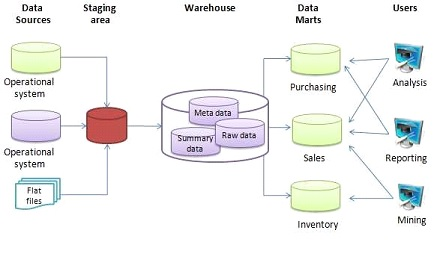
\includegraphics[height=0.5\textheight]{Data_warehouse_architecture} \\
A data warehouse is a system that stores highly structured information from various sources. Data warehouses typically store current and historical data from one or more systems

  \note{
	The next stop is Data Warehouse.
	Historically, data warehouses appeared as a solution for a problem when you need to accumulate multiple data sources for some kind of analysis. \\
	You might be wondering, "Is a data warehouse a database?" Yes, a data warehouse is a giant database that is optimized for analytics.
	So you create a large database and accumulate all data sources there. That simple \\
	And also there is a Data Lake approach which is similar
  }
\end{frame}
\begin{frame}
  \frametitle{Data Lake}
  \centering\LARGE
  Data Lake is another answer for the same problem:
  \begin{columns}
	\begin{column}{0.7\textwidth}
	  \begin{itemize}{}
		\item Large amounts of data (historical data)
		\item Multiple data sources
		\item Variety of clients
		\item Filtering, aggregation, cleansing required
	  \end{itemize}
	\end{column}
  \end{columns}
  \note {
	It solves the same issue. \\
  The issue when you have:
	Data you have required cleansing, filtering, aggregation
	But there are differences
	And the main one is philosophy of a Data Lake approach
  }
\end{frame}
% \begin{frame}
%   \frametitle{Data Lake Philosophy}
%   \LARGE\centering
%   Load First, Think Later
% % Data Lake vs Data Warehouse = Load First, Think Later vs Think First, Load Later
%   \note{
% 	That's it. You have data, you load it and then decide how you process. You load whole data stream. You don't care about schema. We can decide later.
% 	So now it's easy to understand that compared to warehouse
%   }
% \end{frame}
\begin{frame}
  \frametitle{Data Lake vs. Data Warehouse}
  \begin{center}
	\large
  \begin{tabular}{ | c || c c | }
	\hline
	* & Data Warehouse & Data Lake\\
	\hline
    Structure & Structured & Unstructured\\
	Clients & Business/Analytics & Business/Analytics/Data Science\\
	Accessibility & More complex & Less Complex\\
	Workflow & ETL & ELT\\
	Strategy & Think then Upload & Upload then Think\\
	\hline
  \end{tabular}
  \end{center}
  \note {
  The most significan one is philosophy: Load First, Think Later
	Don't think, just upload.\\
  Your data is semi-structured, it's ok. Upload
  You don't know what fields you need later for downstream processing? Never mind, upload, we can decide later on\\
  Done. selling point.\\
	But also compared to Data Warehouse Data Lake has
  }
\end{frame}
\begin{frame}
  \frametitle{Benefits}
  \centering\LARGE
  \begin{columns}
	\begin{column}{0.7\textwidth}
	  \begin{itemize}{}
		\item Cost effective storage
		\item Wide amount of tools available
			  \pause
    \item Reduced vendor lock
		\item Central integration point and data mart for your organization
		\item Centralized Governance
	  \end{itemize}
	\end{column}
  \end{columns}
  \note{
	When we use Data Warehouse we usually locked with technology stack it provides. When we work with plain csv and JSON files it's up to you to decide what instruments to use
	What's why a lot of organizations have Data Lakes
	We want to try the same approach. Data Lake.
  We're working on a blueprint
  }
\end{frame}
\begin{frame}
  \frametitle{Data Lake Blueprint}
  \centering\LARGE
  \begin{columns}
	\begin{column}{0.9\textwidth}
	  \begin{itemize}
    \item Design something that looks like a Data Lake
		\item Define common procedures: Load, Transform, Export
		\item Clarify data Storage format and structure
	\pause
		\item Recommend tools and frameworks
		\item Provide developer guidelines
		\item Introduce Governance
	  \end{itemize}
	\end{column}
  \end{columns}
  \note{
	We're working on a Blueprint where we want to define... \\
  Our concept is quite simple
  }
\end{frame}
\begin{frame}
  \frametitle{What we have}
		\centering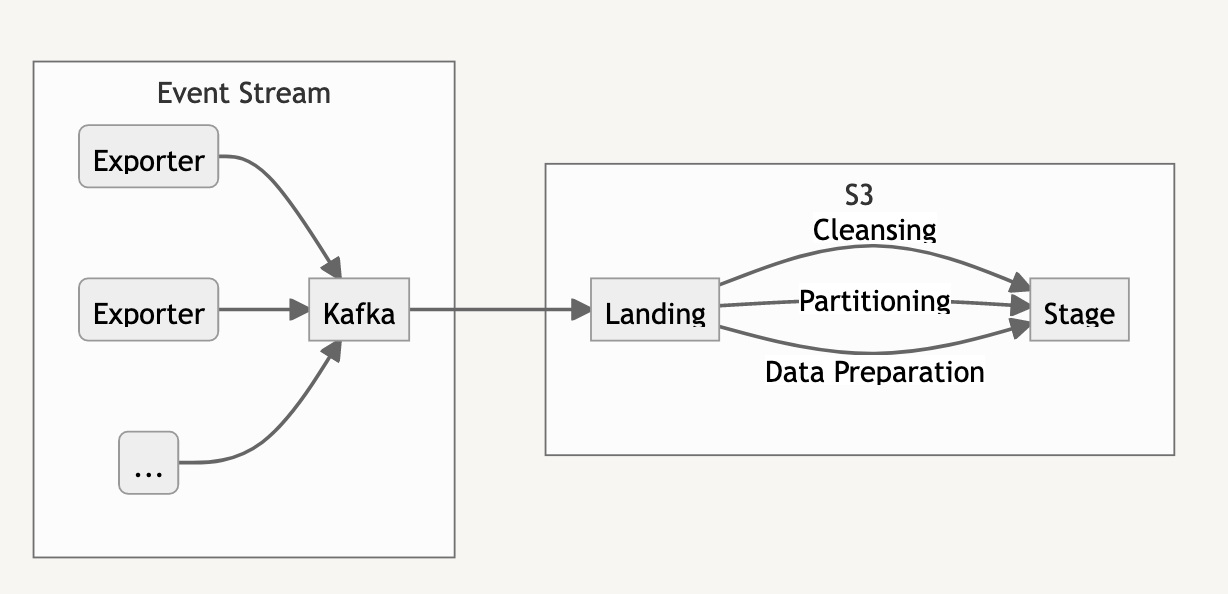
\includegraphics[height=0.9\textheight]{s3datalake} \\
  \note{
	Our concept is not new and it should be familiar to you
	We have S3 as Data Storage and Kafka as a primary interface that you can use to dump your data source into the data lake.
  }
\end{frame}
\begin{frame}
  \frametitle{What we are working on}
	\centering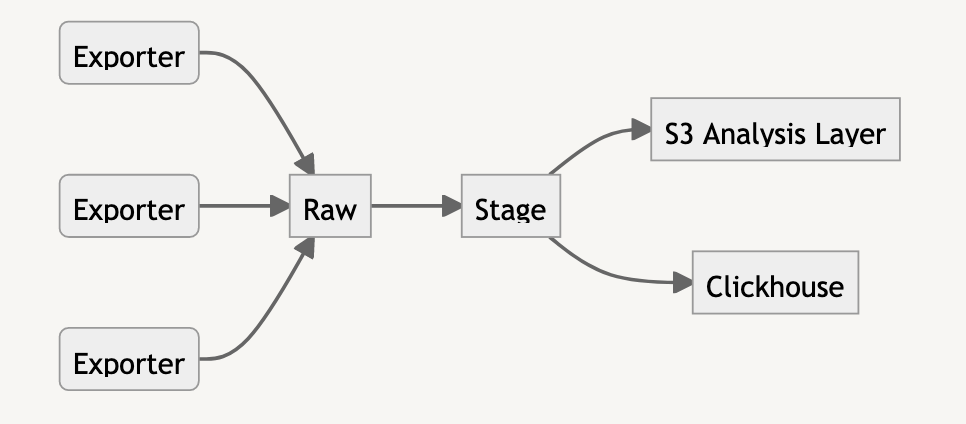
\includegraphics[height=0.3\textheight]{s3datalake1} \\
  \centering\large
  \begin{columns}
	\begin{column}{0.7\textwidth}
	  \begin{itemize}
		\item Start initiative approval process
		\item Find integration points with the current projects/processes
		\item Governance: Retention/Archiving/Backup, Data Catalog, ...
		\item Tools evaluation
	  \end{itemize}
	\end{column}
	\pause
	\begin{column}{0.3\textwidth}
	  \begin{itemize}
		\item Procedures
			  \begin{itemize}
				\item Daily Uploads
				\item Hourly Uploads
        \item ETL
			  \end{itemize}
		\item Basic ETL
		\item Data ingestion unification
	  \end{itemize}
	\end{column}
  \end{columns}
  \note{
	Our current scope is \\
  I personally look for someone who can approve this initiative. \\
  Make it formal\\
  it's all started like an idea. Now we have something to show. Should we proceed? \\
	We have 2 projects candidates to begin with and want to create a POC. \\
  What we need
  }
\end{frame}
\begin{frame}
  \centering\LARGE
  \frametitle{What we need}
  \begin{columns}
    \begin{column}{0.8\textwidth}
      \begin{itemize}
        \item Engineers and budget =)
        \item Public awareness
        \item Facilitation
      \end{itemize}
    \end{column}
  \end{columns}
  \note{
    I want to concentrate as much data sources as possible in this data lake.\\
    that's how we can get profit out of it
  }
\end{frame}
\begin{frame}
  \centering\LARGE
  Thank you
\end{frame}
\end{document}

% We are going to explain unified processes of:
% - Data Extraction
% - Data Cleaning
% - Data Transformation
% - Data Loading and Refreshing


%  	Data Lake 	Data Warehouse
% Data Structure 	Raw 	Processed
% Purpose of Data 	Not yet determined 	Currently in use
% Users 	Data scientists 	Business professionals
% Accessibility 	Highly accessible and quick to update 	More complicated and costly to make changes

% Key differences:
%     Data Lake stores all data irrespective of the source and its structure whereas Data Warehouse stores data in quantitative metrics with their attributes.
%     Data Lake is a storage repository that stores huge structured, semi-structured and unstructured data while Data Warehouse is blending of technologies and component which allows the strategic use of data.
%     Data Lake defines the schema after data is stored whereas Data Warehouse defines the schema before data is stored.
%     Data Lake uses the ELT(Extract Load Transform) process while the Data Warehouse uses ETL(Extract Transform Load) process.
%     Comparing Data lake vs Warehouse, Data Lake is ideal for those who want in-depth analysis whereas Data Warehouse is ideal for operational users.

% Database:
% A database is a collection of data or information.
% Warehouse
% A data warehouse is a system that stores highly structured information from various sources. Data warehouses typically store current and historical data from one or more systems
% Data warehouses store large amounts of current and historical data from various sources. They contain a range of data, from raw ingested data to highly curated, cleansed, filtered, and aggregated data.



% Data Lake
% A data lake is a repository of data from disparate sources that is stored in its original format
% Is a data lake a database? Kind of

% Data Lake is:

% We are building Bluepring
% What we have:
% - 1

% Scope of the first iteration is:
